\documentclass{beamer}
\usepackage{minted}
\usepackage{transparent}
\usetheme{Boadilla}
\usepackage[ddmmyyyy]{datetime}
\usecolortheme{beaver}
\setbeamercovered{transparent}
\setbeamertemplate{caption}{\raggedright\insertcaption\par}
\newcommand\Fontvi{\fontsize{9.5}{7.2}\selectfont}
\usepackage[T1]{fontenc}

\begin{document}

\title[Sicurezza binaria di WebAssembly]{Analisi della sicurezza binaria di WebAssembly}
\author{Alessandro Arata}
\date{17 Settembre 2021}
\begin{frame}
\centerline{
\includegraphics[width=4cm,height=4cm,keepaspectratio]{images/unige.png}}
  \titlepage
  \centerline{Relatore: Prof. Giovanni Lagorio}
\end{frame}

\begin{frame}
  \frametitle{WebAssembly}
  \begin{columns}
    \begin{column}{0.6\textwidth}
      \begin{itemize}
        \item linguaggio bytecode 
        \item tempi di esecuzione rapidi
        \item formato portabile
      \pause
      \item \textbf{target di compilazione}
      \pause
      \item eseguito su \textbf{browser} o in backend 
      \end{itemize}
    \end{column}
    \begin{column}{0.4\textwidth}
      \centerline{
\includegraphics[width=3cm,height=3cm,keepaspectratio]{images/logo.png}}
      \newline\newline\newline
      \centerline{
\includegraphics[width=4cm,height=4cm,keepaspectratio]{images/browser-logos.png}}
    \end{column}
  \end{columns}
\end{frame}

\begin{frame}[fragile]
  \frametitle{hello-world.wat}
  \Fontvi
  \begin{minted}{c}
    puts("Hello, world!");
  \end{minted}

  \vspace{0.2in}
  \centerline{corrisponde nel formato assembly di WebAssembly  (\textbf{.wat}) a}
  \vspace{0.2in}

  \pause

  \begin{minted}{wat}
    (module
      ;; Imports from JavaScript namespace and log function
      (import  "console"  "log" (func  $log (param  i32  i32)))
      ;; Import 1 page of memory
      (import  "js"  "mem" (memory  1))
      ;; Data section of our module
      (data (i32.const 0) "Hello, world!")
      ;; Function declaration: Exported as helloWorld(), no arguments
      (func (export  "helloWorld")
        ;; pass offset 0 to log
        i32.const 0
        ;; pass length 13 to log (strlen of sample text)
        i32.const 13          
        call  $log
      )
    ) 
  \end{minted}
\end{frame}

\begin{frame}
  \frametitle{Tipi e gestione della memoria di WebAssembly}
  \begin{columns}
    \begin{column}{0.6\textwidth}
  \begin{itemize}
    \item staticamente tipato
      \begin{itemize}
        \item \textbf{i32/64} e \textbf{f32/64}
      \end{itemize}
    \pause
    \item stack delle chiamate gestito dalla macchina virtuale
    \pause
    \item tipi non primitivi salvati \newline nella \textbf{memoria lineare}
    \begin{itemize}
      \item gestita dal programma
    \end{itemize}
  \end{itemize} 
  \end{column}
  \begin{column}{0.4\textwidth}
  \centerline{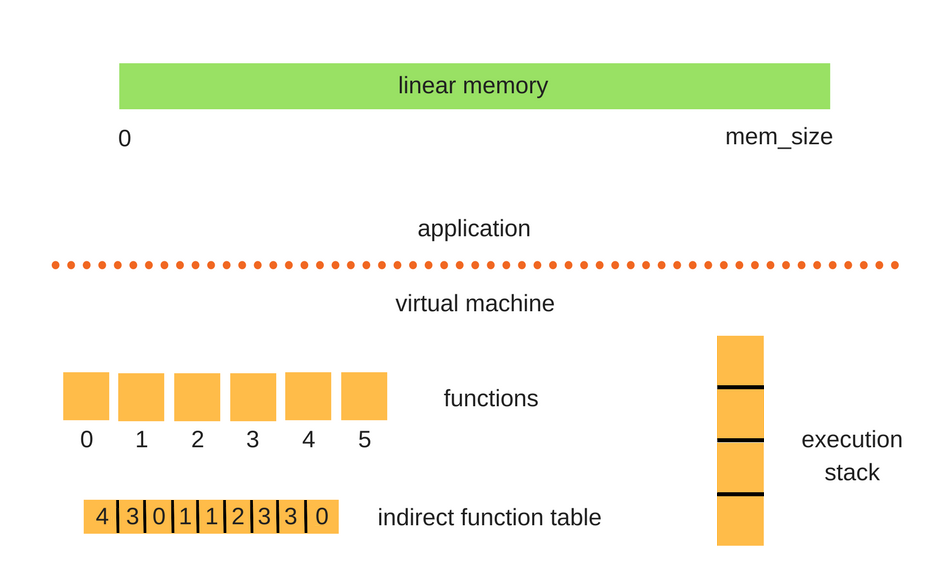
\includegraphics[width=10cm,height=3.5cm,keepaspectratio]{images/linmem.png}}
    \end{column}
  \end{columns}
\end{frame}

\begin{frame}
  \frametitle{Memoria lineare}
  \begin{columns}
    \begin{column}{0.6\textwidth}
      \begin{itemize}
        \item array \textbf{globale} di byte
        \pause
        \item divisa in \textbf{regioni} per heap, stack e dati statici
        \pause
        \item sia leggibile che scrivibile ma non eseguibile 
        \pause
        \item ogni puntatore compreso tra \newline [0, mem\_max] è valido 
      \end{itemize}
    \end{column}
    \begin{column}{0.4\textwidth}
      \centerline{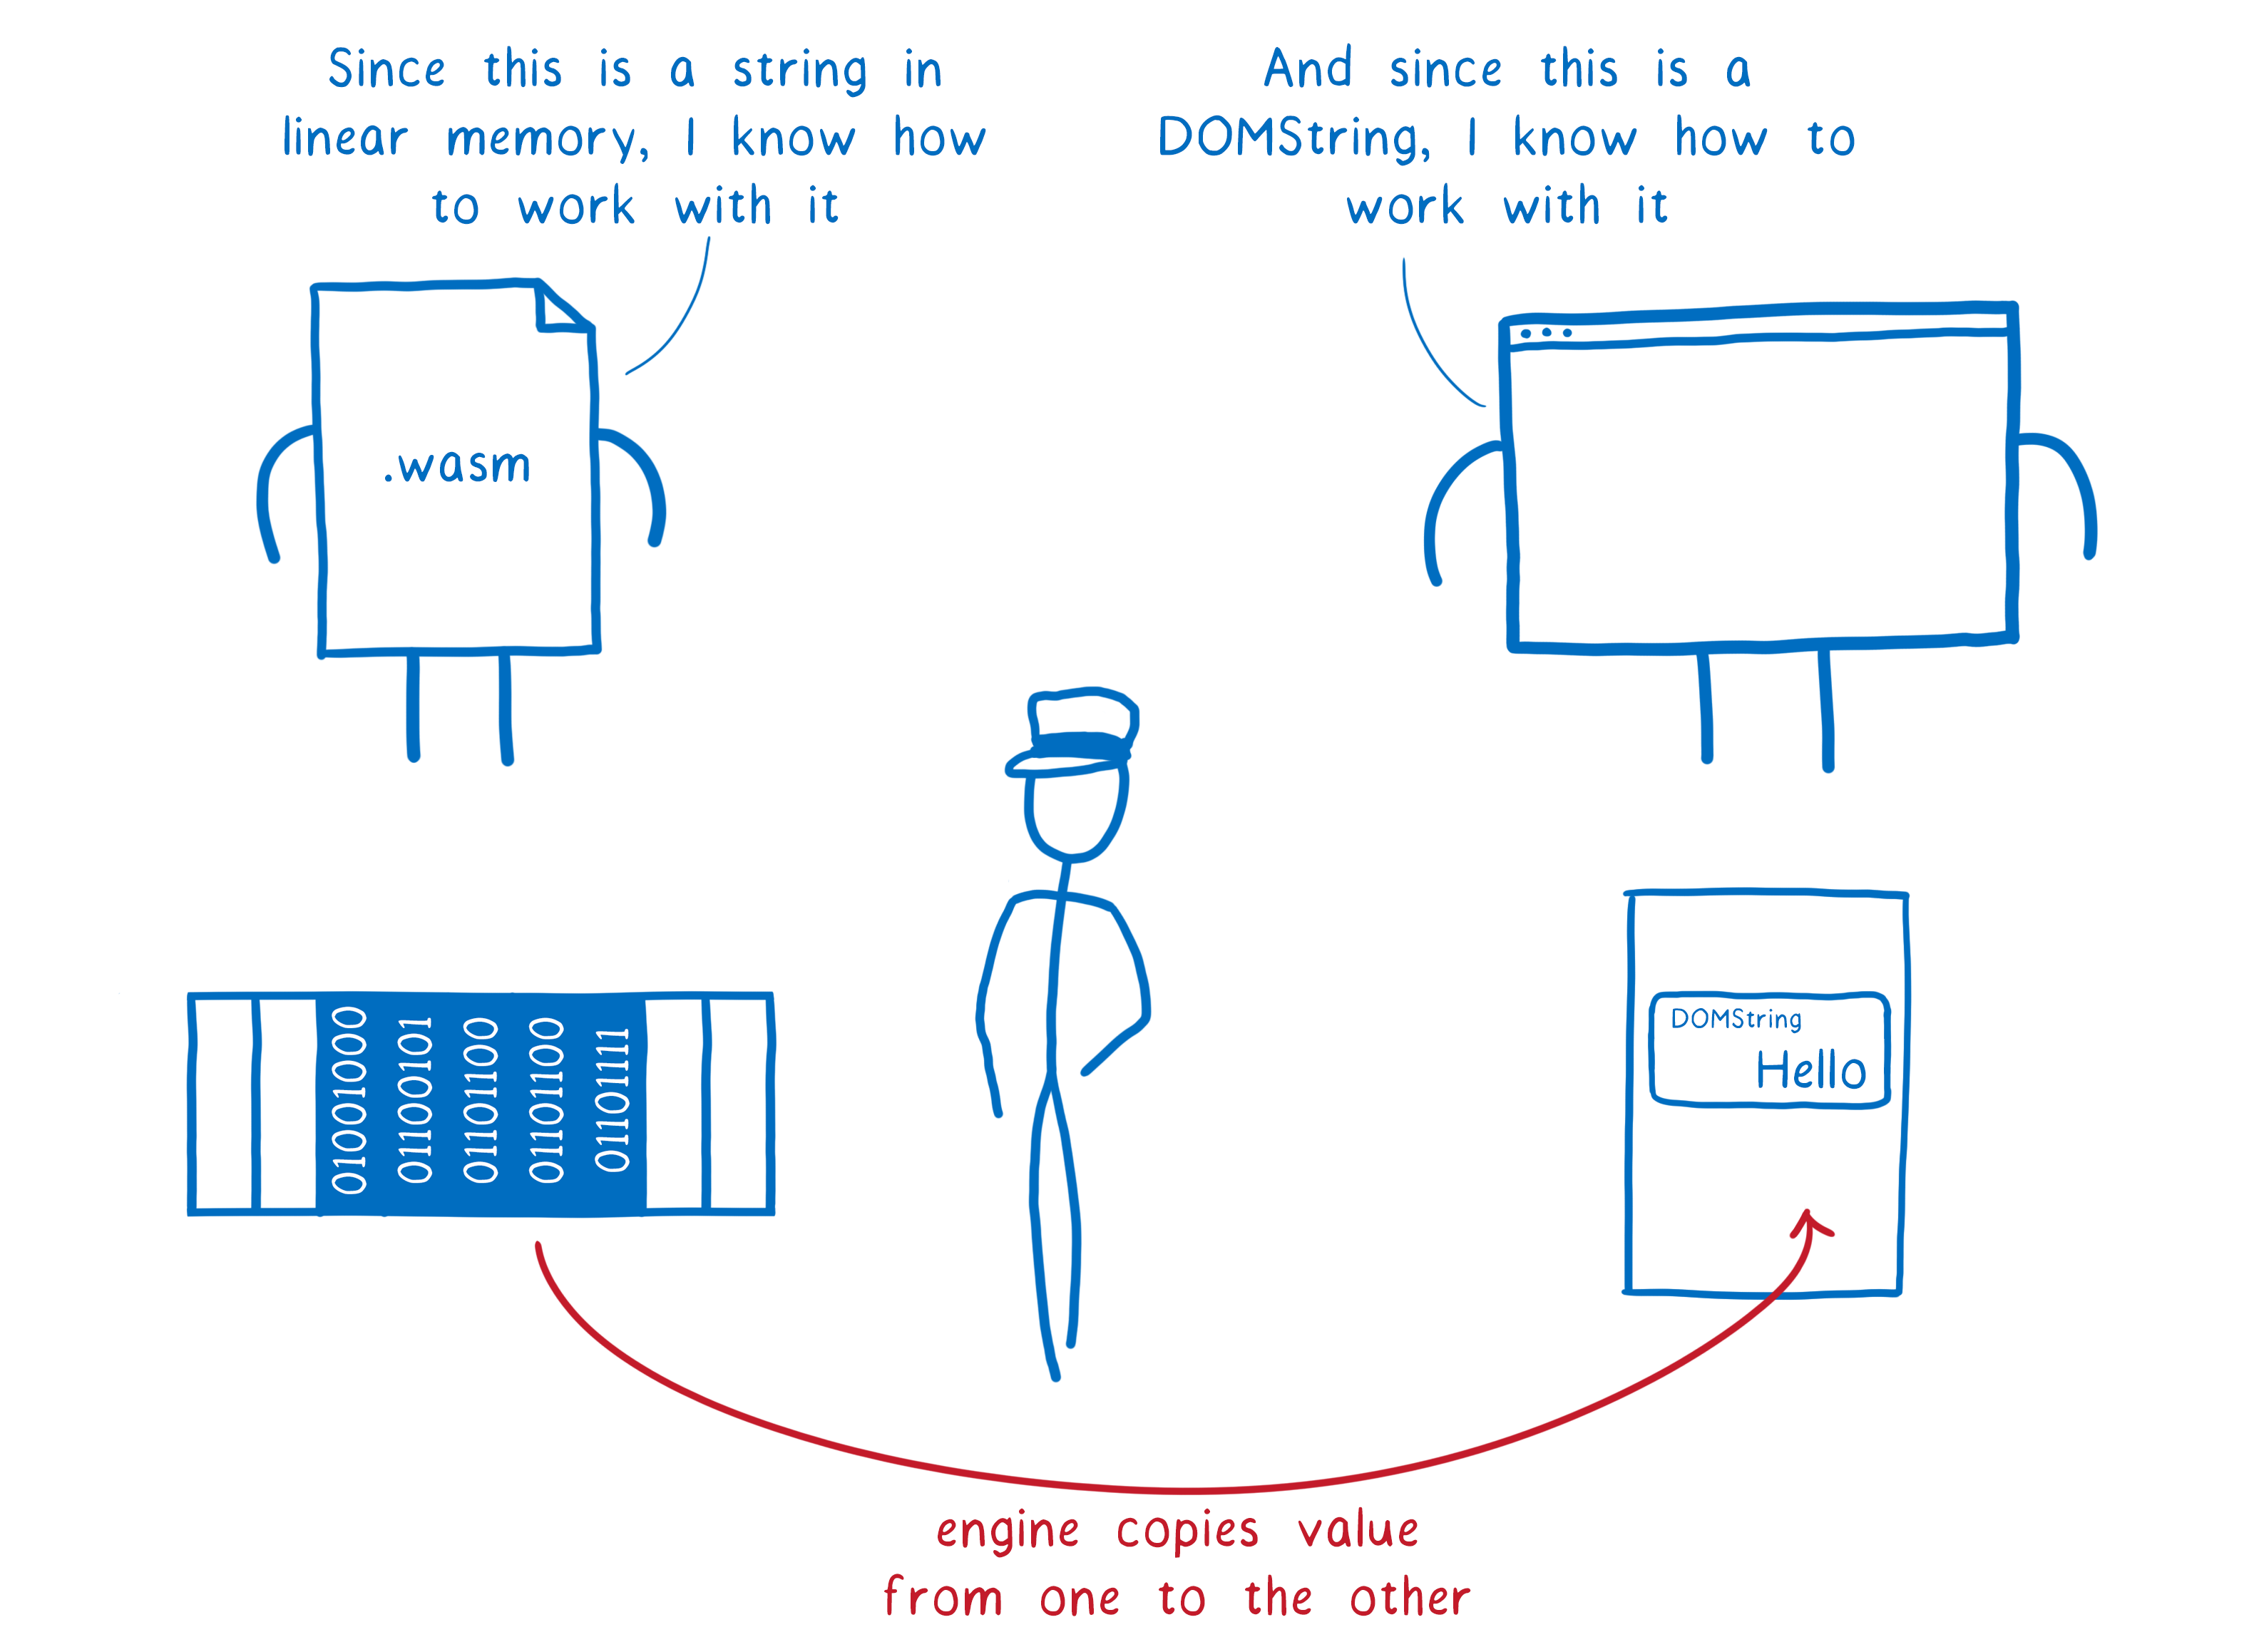
\includegraphics[width=9cm,height=4cm,keepaspectratio]{images/memman.png}}
    \end{column}
  \end{columns}
\end{frame}

\begin{frame}
  \frametitle{Principali mitigazioni nei binari nativi}
      \begin{itemize}
        \item \textbf{Address Space Layout Randomization} (ASLR)     
        \pause
        \item \textbf{Guard pages}   
        \pause
        \item \textbf{Stack canaries}
        \pause 
        \item \textbf{Non-executable stack} (NX)
    \pause 
    \item esistono sezioni non scrivibili (per i dati costanti)
    \pause
    \item aree di memoria del processo potrebbero non essere mappate
      \begin{itemize}
        \item page fault
      \end{itemize}
  \end{itemize}
\end{frame}



\begin{frame}
  \frametitle{Sicurezza binaria della memoria lineare} 
  \begin{columns}
    \begin{column}{0.5\textwidth}
  \begin{itemize}
    \item \textcolor{red}{\textbf{Address Space Layout Randomization} (ASLR)} 
    \pause
    \item \textcolor{red}{\textbf{Guard pages}}   
    \pause
    \item \textcolor{red}{\textbf{Stack canaries}}
    \pause 
    \item \textcolor{green}{\textbf{Non-executable stack} (NX)}
    
      \pause
    \end{itemize}
    \end{column}
    \begin{column}{0.5\textwidth}
      \centerline{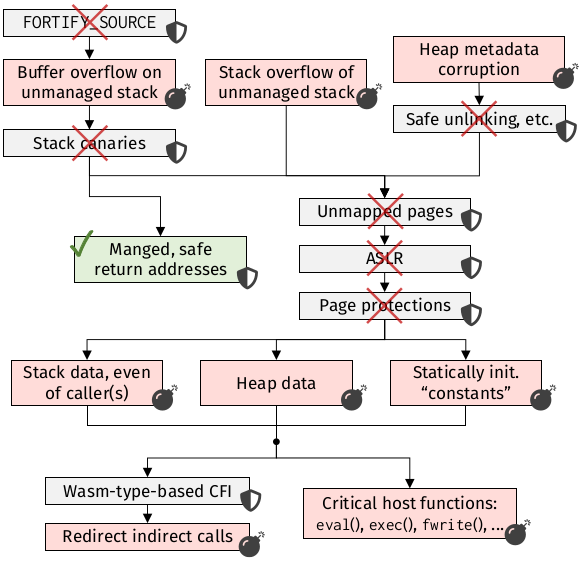
\includegraphics[width=10cm,height=5cm,keepaspectratio]{images/mitigations.png}}
    \end{column}
  \end{columns}

  \vspace{0.15in}
    \begin{itemize}
    \item \textcolor{red}{esistono sezioni non scrivibili (per i dati
      costanti)}
    \pause
    \item \textcolor{red}{aree di memoria del processo potrebbero non essere
    mappate}
      \begin{itemize}
        \item \textcolor{red}{page fault}
      \end{itemize}
  \end{itemize}
\end{frame}

\begin{frame}
  \frametitle{Primitiva di attacco: buffer overflow}
  \begin{columns}
    \begin{column}{0.6\textwidth}
      \begin{itemize}
        \item l'attaccante scrive al di fuori del buffer allocato         
        \begin{itemize}
          \item si possono sovrascrivere variabili locali o indirizzi di
            ritorno
        \end{itemize}
        \pause
        \item \textbf{gets()} e \textbf{strcpy()} permettono questo tipo di attacco
        \pause
      \end{itemize} 
        
    \end{column}
    \begin{column}{0.4\textwidth}
      \centerline{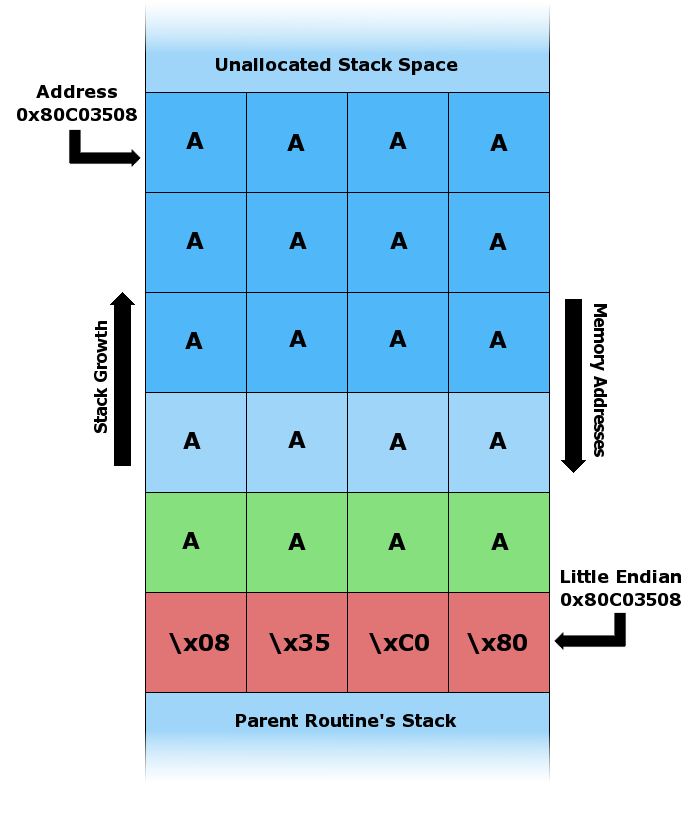
\includegraphics[width=9cm,height=5.5cm,keepaspectratio]{images/stack.png}}
    \end{column}
  \end{columns}
  \vspace{0.15in}
  Cosa succede se un programma \textbf{vulnerabile} a un buffer overflow viene compilato
  in WebAssembly?
\end{frame}

\begin{frame}[fragile]
  \frametitle{Sovrascrivere dati ``costanti''}
  \Fontvi
  \begin{minted}{c}
    char *other_data = "AAAA";

    static char *safe_script = 
      "console.log('this should be safe, shouldn\\'t it?')";


    int main() {
       
      emscripten_run_script(safe_script);
    
    }


    void vuln(const char* input) {
    
      strcpy(other_data, input);

    }
  \end{minted}
\end{frame}

\begin{frame}
  \frametitle{Sovrascrivere dati ``costanti''}
  \begin{columns}
    \begin{column}{0.55\textwidth}
      \begin{itemize}
        \item variabili statiche salvate nella regione \textbf{data}
        \pause
        \item \textbf{strcpy()} non effettua controlli sulla dimensione dell'input
          \begin{itemize}
            \item si sovrascrivono dati sullo stack
          \end{itemize}
          \pause
        \item l'overflow dallo stack scrive nella regione \textbf{data}
        \pause
        \begin{itemize}
      \item si sovrascrive \textbf{safe\_script} 
        \end{itemize}
      \item \textbf{XSS} e \textbf{RCE}  
      \end{itemize}
      
    \end{column}
    \begin{column}{0.45\textwidth}
      \begin{figure}[htbp]
        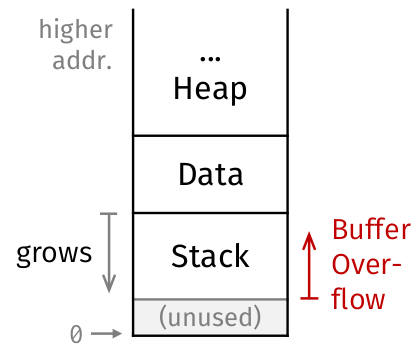
\includegraphics[width=4cm,height=6cm,keepaspectratio]{images/memory_layout.png}
        \newline
        \begin{figure}
          \only<-3>{\transparent{0.4}{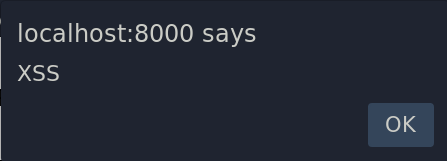
\includegraphics[width=4cm,height=6cm,keepaspectratio]{images/xss.png}}\vfill}
           
          \only<4>{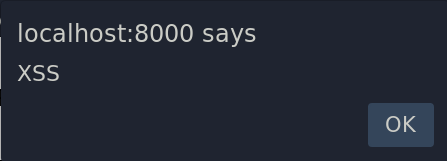
\includegraphics[width=4cm,height=6cm,keepaspectratio]{images/xss.png}}
          \caption{Chiamando \textbf{vuln()} con la stringa
          ";;;;;;;;;;;;;;;;;;;;;;;;;;;;;;;;;alert('XSS')"}
        \end{figure}
        \end{figure}
    \end{column}
  \end{columns}
\end{frame}

\begin{frame}[fragile]
  \frametitle{Heap overflow (a partire dallo stack)}
  \begin{itemize}
    \item similmente è possibile sovrascrivere dati sullo heap
    \pause
    \item \textbf{libpng} contiene un buffer overflow 
  \pause
  \end{itemize}
  \vspace{0.15in}
  \begin{minted}{c++}
    std::string img_tag = 
      "<img src='data:image/png;base64,";
    pnm2png("input.pnm", "output.png");        
    img_tag += file_to_base64("output.png") + "'>";
    emcc::global("document").call("write", img_tag);
  \end{minted}
  \vspace{0.15in}
  \pause
  \begin{itemize}
    \item si può sovrascrivere \textbf{img\_tag} nello heap    
    \begin{itemize}
      \item \textbf{XSS}
    \end{itemize}
  \end{itemize}
\end{frame}

\begin{frame}
  \frametitle{Heap overflow (a partire dallo stack)}
  \Fontvi 
  \begin{columns}
    \begin{column}{0.5\textwidth}
      \begin{figure}
        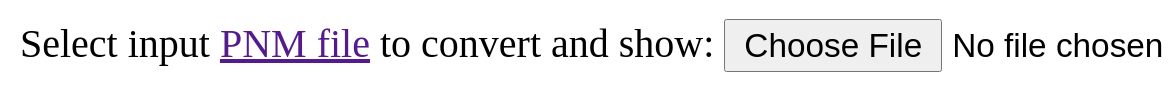
\includegraphics[width=5cm,height=6cm,keepaspectratio]{images/site.png}
        \caption{Il sito chiede all'utente un'immagine in input: non vengono
        fatti controlli sul tipo di file.} 
      \end{figure} 
      \pause
      \begin{figure}
        \only<1>{\transparent{0.4}{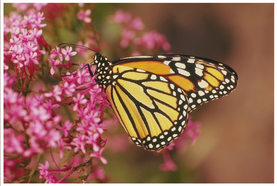
\includegraphics[width=4cm,height=4cm,keepaspectratio]{images/butfly.png}}\vfill}
        \only<2->{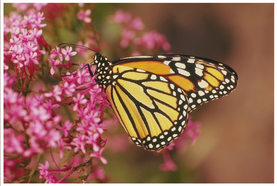
\includegraphics[width=4cm,height=4cm,keepaspectratio]{images/butfly.png}}
        \caption{Se l'utente immette un'immagine, questa viene convertita
        e mostrata nel browser.}
      \end{figure} 
    \pause
    \end{column}
    \begin{column}{0.5\textwidth}
      Utilizzando come payload un file contenente
      \newline\newline\newline
      AAAAAAAAAAAAAAAAAAAAAAAA...
      <script>alert('XSS')</script><!- -
      \newline\newline\newline
      \pause
      si effettua un overflow nello stack che permette di sostituire al tag
      \textbf{<img>} il tag \textbf{<script>} nello heap: questo provoca un attacco di
      tipo XSS.
      \newline\newline\newline
      \only<-3>{\transparent{0.4}{\centerline{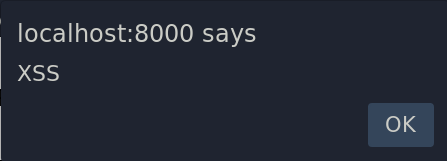
\includegraphics[width=5.5cm,height=5.5cm,keepaspectratio]{images/xss.png}}}\vfill}
    \only<4>{\centerline{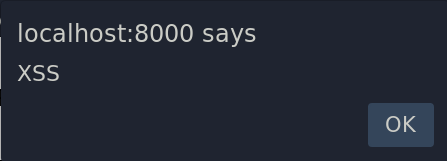
\includegraphics[width=5.5cm,height=5.5cm,keepaspectratio]{images/xss.png}}}

    \end{column}

  \end{columns}
\end{frame}


\begin{frame}
  \frametitle{Conclusioni}
  WebAssembly ha

  \vspace{0.2in}
  \begin{itemize}
    \item reintrodotto vulnerabilità precedentemente mitigate 
    \pause
    \item introdotto nel web vulnerabilità legate ai binari
      \begin{itemize}
        \item buffer/heap overflow
        \item format string
        \item ...
      \end{itemize}
    \pause
    \item reso possibili nuovi tipi di attacco
      \begin{itemize}
        \item sovrascrivere dati ``costanti''
        \item sovrascrivere dati di una regione a partire da un'altra
      \end{itemize}
  \end{itemize}
\end{frame}

\begin{frame}
  \frametitle{Bibliografia}
  \begin{enumerate}
    \item Daniel Lehmann, Johannes Kinder, Michael Pradel: \emph{"Everything Old is New Again:
      Binary Security of WebAssembly"}
    \item Brian McFadden, Tyler Lukasiewicz, Jeff Dileo, Justin Engler:
      \emph{"Security Chasms of WASM"}
  \end{enumerate}
\end{frame}

\end{document}
